\documentclass[dutch]{../khlslides}
\usepackage{graphicx}
\usepackage{pxfonts}
\usepackage{tikz}
\usepackage{calc}
\usepackage{fourier}

\usetikzlibrary{calc,shadows,decorations.markings}


\title{Relaties}
\logo{
\includegraphics[height=0.5cm]{../KHL.jpg}}
\institute[KHL]{KHLeuven}


\newcommand{\element}[3][]{
  \draw[fill=black] (#2) circle (.05);
  \node[anchor=south west,#1] at (#2) {#3};
}

\newcommand{\union}{\cup}
\newcommand{\intersect}{\cap}

\newcommand{\leftellipse}{(-2,0) ellipse (3cm and 2cm)}
\newcommand{\rightellipse}{(2,0) ellipse (3cm and 2cm)}

\pgfkeys{
  /tikz/.cd,
}


\newcommand{\axes}{
  \path[use as bounding box] (-.5,-.5) rectangle (4,4);
  \draw[step=3cm,gray,thin] (-.5,-.5) grid (4,4);
  \draw[thin,->] (-.5,0) -- (4,0) node[at end,above left] {$A$};
  \draw[thin,->] (0,-.5) -- (0,4) node[at end,left] {$B$};
}


\begin{document}

\maketitle

\section{Relaties}

\frame{ \tableofcontents[currentsection] }

\begin{frame}
  \frametitle{Wat Zijn Relaties?}
  \begin{center}
    \begin{tikzpicture}[decoration={markings,mark=at position 0.5 with {\arrow{>}}}]
      \draw[thick] (-3,0) ellipse (2cm and 3cm); \node at (-4,3) {A};
      \draw[thick] (3,0) ellipse (2cm and 3cm); \node at (4,3) {B};

      \foreach \i in {-1.5,...,1.5} {
        \draw[fill=black] (-3,\i) circle (.05);
      }

      \foreach \i in {-1,...,1} {
        \draw[fill=black] (3,\i) circle (.05);
      }

      \only<2>{
        \draw[thick,postaction={decorate}] (-3,1.5) -- (3,1);
        \draw[thick,postaction={decorate}] (-3,.5) -- (3,0);
        \draw[thick,postaction={decorate}] (-3,-.5) -- (3,-1);
        \draw[thick,postaction={decorate}] (-3,-1.5) -- (3,-1);
      }

      \only<3>{
        \draw[thick,postaction={decorate}] (-3,1.5) -- (3,0);
        \draw[thick,postaction={decorate}] (-3,.5) -- (3,0);
        \draw[thick,postaction={decorate}] (-3,-.5) -- (3,0);
        \draw[thick,postaction={decorate}] (-3,-1.5) -- (3,0);
      }

      \only<4>{
        \draw[thick,postaction={decorate}] (-3,.5) -- (3,1);
        \draw[thick,postaction={decorate}] (-3,.5) -- (3,-1);
        \draw[thick,postaction={decorate}] (-3,-.5) -- (3,1);
        \draw[thick,postaction={decorate}] (-3,-.5) -- (3,-1);
      }
    \end{tikzpicture}
  \end{center}
\end{frame}

\begin{frame}
  \frametitle{Relaties}
  \begin{itemize}
    \item Relatie van verzameling A naar verzameling B
    \item A heet \emph{bronverzameling} of \emph{domein}
    \item B heet \emph{doelverzameling} of \emph{bereik}
    \item Een relatie maakt associaties
    \item Elk element uit A wordt met 0+ elementen uit B verbonden
  \end{itemize}
  \vskip5mm
\end{frame}

\begin{frame}
  \frametitle{Voorbeelden}
  \structure{Studenten en Vakken}
  \begin{itemize}
    \item Domein: verzameling studenten
    \item Bereik: verzameling vakken
    \item Relatie: student ``volgt'' vak
  \end{itemize}
  \vskip5mm
  \structure{Acteurs en Films}
  \begin{itemize}
    \item Domein: verzameling acteurs
    \item Bereik: verzameling films
    \item Relatie: acteur ``speelt mee in'' film
  \end{itemize}
\end{frame}

\begin{frame}
  \frametitle{Wiskundige Definitie}
  \begin{overprint}
    \onslide<1>
    \[
      A \qquad B
    \]
    \onslide<2>
    \[
      A \times B
    \]
    \onslide<3>
    \[
      R \subset A \times B
    \]
  \end{overprint}
  \begin{center}
    \begin{tikzpicture}[decoration={markings,mark=at position 0.5 with {\arrow{>}}}]
      \draw[thick] (-3,0) ellipse (2cm and 3cm); \node at (-4,3) {A};
      \draw[thick] (3,0) ellipse (2cm and 3cm); \node at (4,3) {B};

      \foreach \i in {-1.5,...,1.5} {
        \draw[fill=black] (-3,\i) circle (.05);
      }

      \foreach \i in {-1,...,1} {
        \draw[fill=black] (3,\i) circle (.05);
      }

      \only<2>{
        \foreach \i in {-1.5,...,1.5} {
          \foreach \j in {-1,...,1} {
            \draw[thick,postaction={decorate}] (-3,\i) -- (3,\j);
          }
        }
      }

      \only<3>{
        \draw[thick,postaction={decorate}] (-3,1.5) -- (3,1);
        \draw[thick,postaction={decorate}] (-3,.5) -- (3,0);
        \draw[thick,postaction={decorate}] (-3,.5) -- (3,1);
        \draw[thick,postaction={decorate}] (-3,-.5) -- (3,-1);
        \draw[thick,postaction={decorate}] (-3,-1.5) -- (3,-1);
      }
    \end{tikzpicture}
  \end{center}
\end{frame}

\begin{frame}
  \frametitle{Notatie: Opsomming}
  \begin{center}
    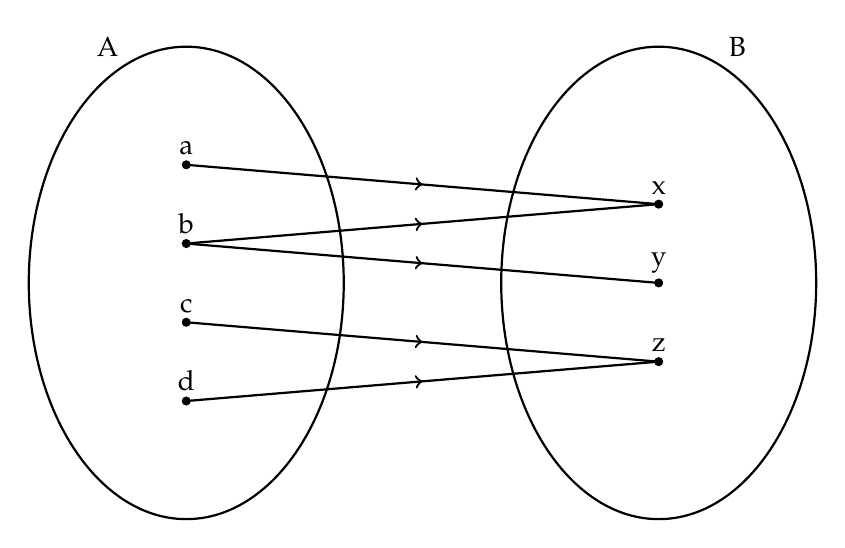
\begin{tikzpicture}[decoration={markings,mark=at position 0.5 with {\arrow{>}}}]
      \draw[thick] (-3,0) ellipse (2cm and 3cm); \node at (-4,3) {A};
      \draw[thick] (3,0) ellipse (2cm and 3cm); \node at (4,3) {B};

      \foreach \i/\c in {-1.5/d,-.5/c,.5/b,1.5/a} {
        \draw[fill=black] (-3,\i) circle (.05);
        \node[above] at (-3,\i) {\c};
      }

      \foreach \i/\c in {-1/z,0/y,1/x} {
        \draw[fill=black] (3,\i) circle (.05);
        \node[above] at (3,\i) {\c};
      }

      \draw[thick,postaction={decorate}] (-3,1.5) -- (3,1);
      \draw[thick,postaction={decorate}] (-3,.5) -- (3,0);
      \draw[thick,postaction={decorate}] (-3,.5) -- (3,1);
      \draw[thick,postaction={decorate}] (-3,-.5) -- (3,-1);
      \draw[thick,postaction={decorate}] (-3,-1.5) -- (3,-1);
    \end{tikzpicture}
  \end{center}
  \[
    R = \left\{
          (a, x), (b, x), (b, y), (c, z), (d, z)
        \right\}
  \]
\end{frame}

\begin{frame}
  \frametitle{Oefening}
  Geef door opsomming en teken de grafiek
  \[
      \left\{ \; (x, y)  \;|\; (x, y) \in \mathbb{Z}^2, y = x^2 \right\}
  \]
\end{frame}

\begin{frame}
  \frametitle{Oefening}
  Geef door opsomming
  \[
      f : \mathbb{Z}^2 \rightarrow \mathbb{Z} : (x, y) \mapsto x \cdot y
  \]
\end{frame}

\begin{frame}
  \frametitle{Notaties}
  \begin{itemize}
    \item Opsomming
    \item Tabel
    \item Venn-diagram
    \item Grafische voorstelling in 2D-vlak
    \item Functievoorschrift
    \item Algoritme
  \end{itemize}
\end{frame}

\section{Indeling op basis van domein}

\subsection{Functies}
\frame{ \tableofcontents[currentsubsection] }


\begin{frame}
  \frametitle{Functies}
  \begin{center}
    Functies: maximum \'e\'en pijl vanuit elk bronelement
  \end{center}
  \begin{center}
    \begin{tikzpicture}[decoration={markings,mark=at position 0.5 with {\arrow{>}}}]
      \draw[thick] (-3,0) ellipse (2cm and 3cm); \node at (-4,3) {A};
      \draw[thick] (3,0) ellipse (2cm and 3cm); \node at (4,3) {B};

      \foreach \i in {-1.5,...,1.5} {
        \draw[fill=black] (-3,\i) circle (.05);
      }

      \foreach \i in {-1,...,1} {
        \draw[fill=black] (3,\i) circle (.05);
      }

      \only<1>{
        \draw[thick,postaction={decorate}] (-3,1.5) -- (3,1);
        \draw[thick,postaction={decorate}] (-3,-.5) -- (3,-1);
        \draw[thick,postaction={decorate}] (-3,-1.5) -- (3,-1);
        \node at (0,-2.5) {Functie};
      }

      \only<2>{
        \draw[thick,postaction={decorate}] (-3,1.5) -- (3,1);
        \draw[thick,postaction={decorate}] (-3,-.5) -- (3,0);
        \draw[thick,postaction={decorate}] (-3,-.5) -- (3,-1);
        \draw[thick,postaction={decorate}] (-3,-1.5) -- (3,-1);
        \node at (0,-2.5) {Geen functie};
      }
      \end{tikzpicture}
  \end{center}
\end{frame}

\subsection{Afbeeldingen}
\frame{ \tableofcontents[currentsubsection] }


\begin{frame}
  \frametitle{Afbeelding}
  \begin{center}
    Afbeelding: exact \'e\'en pijl vanuit elk bronelement
  \end{center}
  \begin{center}
    \begin{tikzpicture}[decoration={markings,mark=at position 0.5 with {\arrow{>}}}]
      \draw[thick] (-3,0) ellipse (2cm and 3cm); \node at (-4,3) {A};
      \draw[thick] (3,0) ellipse (2cm and 3cm); \node at (4,3) {B};

      \foreach \i in {-1.5,...,1.5} {
        \draw[fill=black] (-3,\i) circle (.05);
      }

      \foreach \i in {-1,...,1} {
        \draw[fill=black] (3,\i) circle (.05);
      }

      \only<1>{
        \draw[thick,postaction={decorate}] (-3,1.5) -- (3,1);
        \draw[thick,postaction={decorate}] (-3,.5) -- (3,0);
        \draw[thick,postaction={decorate}] (-3,-.5) -- (3,-1);
        \draw[thick,postaction={decorate}] (-3,-1.5) -- (3,-1);
        \node at (0,-2.5) {Afbeelding};
      }

      \only<2>{
        \draw[thick,postaction={decorate}] (-3,1.5) -- (3,1);
        \draw[thick,postaction={decorate}] (-3,.5) -- (3,0);
        \draw[thick,postaction={decorate}] (-3,-.5) -- (3,-1);
        \node at (0,-2.5) {Geen afbeelding};
      }
      \end{tikzpicture}
  \end{center}
\end{frame}

\begin{frame}
  \frametitle{Voorbeelden}
  \begin{center}
    \begin{tabular}{cccc}
      \textbf{Bron} & \textbf{Relatie} & \textbf{Doel} & \textbf{Categorie} \\
      \toprule
      Acteur & speelt mee in & film & \only<2->{\sc relatie} \\
      Persoon & heeft als leeftijd & $\mathbb{N}$ & \only<3->{\sc afbeelding} \\
      Getal & heeft als vierkantswortel & getal & \only<4->{\sc functie} \\
      Pos.\ getal & heeft als vierkantswortel & getal & \only<5->{\sc afbeelding} \\
      Persoon & is koning van & land & \only<6->{\sc functie}
    \end{tabular}
  \end{center}
\end{frame}


\section{Indeling op basis van bereik}
\subsection{Surjectief}

\frame{ \tableofcontents[currentsubsection] }


\begin{frame}
  \frametitle{Surjectief}
  \begin{center}
    Er komt minstens \'e\'en pijl aan in elk doelelement
    
    \begin{tikzpicture}[decoration={markings,mark=at position 0.5 with {\arrow{>}}}]
      \draw[thick] (-3,0) ellipse (2cm and 3cm); \node at (-4,3) {A};
      \draw[thick] (3,0) ellipse (2cm and 3cm); \node at (4,3) {B};

      \foreach \i in {-1.5,...,1.5} {
        \draw[fill=black] (-3,\i) circle (.05);
      }

      \foreach \i in {-1,...,1} {
        \draw[fill=black] (3,\i) circle (.05);
      }

      \only<1>{
        \draw[thick,postaction={decorate}] (-3,1.5) -- (3,1);
        \draw[thick,postaction={decorate}] (-3,.5) -- (3,0);
        \draw[thick,postaction={decorate}] (-3,-.5) -- (3,-1);
        \draw[thick,postaction={decorate}] (-3,-1.5) -- (3,-1);
        \node at (0,-2.5) {Surjectief};
      }

      \only<2>{
        \draw[thick,postaction={decorate}] (-3,1.5) -- (3,1);
        \draw[thick,postaction={decorate}] (-3,.5) -- (3,1);
        \draw[thick,postaction={decorate}] (-3,-.5) -- (3,-1);
        \draw[thick,postaction={decorate}] (-3,-1.5) -- (3,-1);
        \node at (0,-2.5) {Niet surjectief};
      }
      \end{tikzpicture}
  \end{center}
\end{frame}

\subsection{Injectief}

\frame{ \tableofcontents[currentsubsection] }


\begin{frame}
  \frametitle{Injectief}
  \begin{center}
    Er komt maximaal \'e\'en pijl aan in elk doelelement
    
    \begin{tikzpicture}[decoration={markings,mark=at position 0.5 with {\arrow{>}}}]
      \draw[thick] (-3,0) ellipse (2cm and 3cm); \node at (-4,3) {A};
      \draw[thick] (3,0) ellipse (2cm and 3cm); \node at (4,3) {B};

      \foreach \i in {-1.5,...,1.5} {
        \draw[fill=black] (-3,\i) circle (.05);
      }

      \foreach \i in {-1,...,1} {
        \draw[fill=black] (3,\i) circle (.05);
      }

      \only<1>{
        \draw[thick,postaction={decorate}] (-3,1.5) -- (3,1);
        \draw[thick,postaction={decorate}] (-3,-1.5) -- (3,-1);
        \node at (0,-2.5) {Injectief};
      }

      \only<2>{
        \draw[thick,postaction={decorate}] (-3,1.5) -- (3,1);
        \draw[thick,postaction={decorate}] (-3,-.5) -- (3,-1);
        \draw[thick,postaction={decorate}] (-3,-1.5) -- (3,-1);
        \node at (0,-2.5) {Niet injectief};
      }
      \end{tikzpicture}
  \end{center}
\end{frame}


\subsection{Bijectief}

\frame{ \tableofcontents[currentsubsection] }


\begin{frame}
  \frametitle{Bijectief}
  \begin{center}
    Er komt exact \'e\'en pijl aan in elk doelelement
    
    \begin{tikzpicture}[decoration={markings,mark=at position 0.5 with {\arrow{>}}}]
      \draw[thick] (-3,0) ellipse (2cm and 3cm); \node at (-4,3) {A};
      \draw[thick] (3,0) ellipse (2cm and 3cm); \node at (4,3) {B};

      \foreach \i in {-1,...,1} {
        \draw[fill=black] (-3,\i) circle (.05);
      }

      \foreach \i in {-1,...,1} {
        \draw[fill=black] (3,\i) circle (.05);
      }

      \only<1>{
        \draw[thick,postaction={decorate}] (-3,1) -- (3,1);
        \draw[thick,postaction={decorate}] (-3,0) -- (3,0);
        \draw[thick,postaction={decorate}] (-3,-1) -- (3,-1);
        \node at (0,-2.5) {Bijectief};
      }

      \only<2>{
        \draw[fill=black] (3,2) circle (.05);
        \draw[thick,postaction={decorate}] (-3,1) -- (3,1);
        \draw[thick,postaction={decorate}] (-3,0) -- (3,0);
        \draw[thick,postaction={decorate}] (-3,-1) -- (3,-1);
        \node at (0,-2.5) {Niet bijectief};
      }
      \end{tikzpicture}
  \end{center}
\end{frame}

\begin{frame}
  \frametitle{Voorbeelden}
  \begin{center}
    \begin{tabular}{cccc}
      \textbf{Bron} & \textbf{Relatie} & \textbf{Doel} & \textbf{Categorie} \\
      \toprule
      Persoon & is koning van & land & \only<2->{\sc Injectief} \\
      Persoon & is componist van & lied & \only<3->{\sc Surjectief} \\
      Naam & is naam van & persoon & \only<4->{\sc Surjectief} \\
      Naam & is naam van & ster & \only<5->{\sc Bijectief} \\
      Naam & is naam van & ster & \only<6->{\sc Bijectief} \\
      Nat.\ getal & is \'e\'en hoger dan & nat.\ getal & \only<7->{\sc Injectief} \\
      Getal & is vierkantswortel van & getal & \only<8->{\sc Injectief} \\
    \end{tabular}
  \end{center}
  \structure{Geheugensteun}
  \begin{center}
    \begin{tabular}{lc}
      Min.\ 1 aankomende pijl & surjectief \\
      Max.\ 1 aankomende pijl & injectief \\
      Exact 1 aankomende pijl & bijectief \\
    \end{tabular}
  \end{center}
\end{frame}

\begin{frame}
  \frametitle{Injecties, Surjecties en Bijecties}
  \begin{itemize}
    \item Injectie: injectief + afbeelding
          \vskip4mm
    \item Surjectie: surjectief + afbeelding
          \vskip4mm
    \item Bijectie: bijectief + afbeelding
  \end{itemize}
\end{frame}

\begin{frame}
  \frametitle{Oefening 2.9}
  \begin{center}
    relatie, functie, afbeelding, injectie(f), surjectie(f), bijectie(f)
    \vskip1cm
    \begin{tikzpicture}
      \axes
      \draw[thick] (0,0) -- (1,1);
      \draw[thick] (2,2) -- (3,3);
    \end{tikzpicture}
  \end{center}
\end{frame}

\begin{frame}
  \frametitle{Oefening 2.9}
  \begin{center}
    relatie, functie, afbeelding, injectie(f), surjectie(f), bijectie(f)
    \vskip1cm
    \begin{tikzpicture}
      \axes
      \draw[thick] (0,0) to[out=90,in=-90] (3,3);
    \end{tikzpicture}
  \end{center}
\end{frame}

\begin{frame}
  \frametitle{Oefening 2.9}
  \begin{center}
    relatie, functie, afbeelding, injectie(f), surjectie(f), bijectie(f)
    \vskip1cm
    \begin{tikzpicture}
      \axes
      \draw[thick] (1.5,0) -- (1.5,3);
    \end{tikzpicture}
  \end{center}
\end{frame}

\begin{frame}
  \frametitle{Oefening 2.9}
  \begin{center}
    relatie, functie, afbeelding, injectie(f), surjectie(f), bijectie(f)
    \vskip1cm
    \begin{tikzpicture}
      \axes
      \draw[thick] (0,1.5) -- (3,1.5);
    \end{tikzpicture}
  \end{center}
\end{frame}

\begin{frame}
  \frametitle{Oefening 2.9}
  \begin{center}
    relatie, functie, afbeelding, injectie(f), surjectie(f), bijectie(f)
    \vskip1cm
    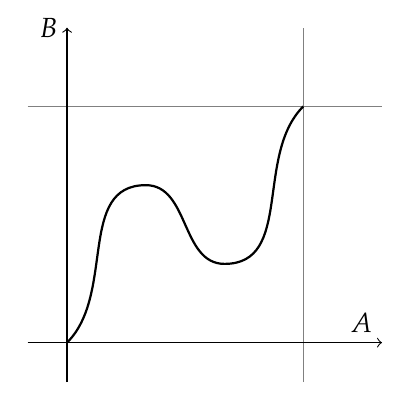
\begin{tikzpicture}
      \axes
      \draw[thick] (0,0) to[out=45,in=180] (1,2) to[out=0,in=180] (2,1) to[out=0,in=225] (3,3);
    \end{tikzpicture}
  \end{center}
\end{frame}

\begin{frame}
  \frametitle{Oefening 2.9}
  \begin{center}
    relatie, functie, afbeelding, injectie(f), surjectie(f), bijectie(f)
    \vskip1cm
    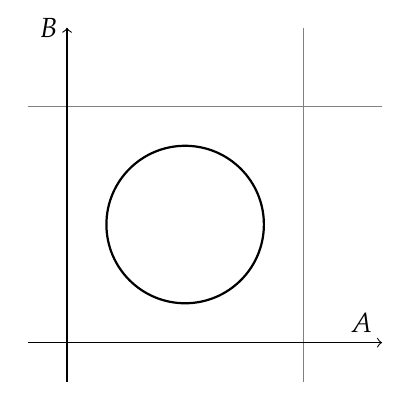
\begin{tikzpicture}
      \axes
      \draw[thick] (1.5,1.5) circle (1cm);
    \end{tikzpicture}
  \end{center}
\end{frame}


\section{Inverse Relatie}

\frame{ \tableofcontents[currentsection] }

\begin{frame}
  \frametitle{Inverse Relatie}
  \begin{center}
    \begin{tikzpicture}[decoration={markings,mark=at position 0.5 with {\arrow{>}}}]
      \draw[thick] (-3,0) ellipse (2cm and 3cm); \node at (-4,3) {A};
      \draw[thick] (3,0) ellipse (2cm and 3cm); \node at (4,3) {B};

      \foreach \i in {-1.5,...,1.5} {
        \draw[fill=black] (-3,\i) circle (.05);
      }

      \foreach \i in {-1,...,1} {
        \draw[fill=black] (3,\i) circle (.05);
      }

      \only<1>{
        \draw[thick,postaction={decorate}] (-3,1.5) -- (3,1);
        \draw[thick,postaction={decorate}] (-3,.5) -- (3,0);
        \draw[thick,postaction={decorate}] (-3,-.5) -- (3,-1);
        \draw[thick,postaction={decorate}] (-3,-1.5) -- (3,-1);
      }

      \only<2>{
        \draw[thick,postaction={decorate}] (3,1) -- (-3,1.5);
        \draw[thick,postaction={decorate}] (3,0) -- (-3,.5);
        \draw[thick,postaction={decorate}] (3,-1) -- (-3,-.5);
        \draw[thick,postaction={decorate}] (3,-1) -- (-3,-1.5);
      }
    \end{tikzpicture}
  \end{center}
\end{frame}

\begin{frame}
  \frametitle{Oefening 2.7}
  Geef de inverse relaties
  \begin{enumerate}
    \item \[ \{ (1, 7), (2, 10), (3, 9) \} \]
    \item \[ f : \mathbb{R} \rightarrow \mathbb{R} : x \mapsto y \;|\; 2 \cdot x + 10 \]
    \item \[ f : \mathbb{R}^+ \rightarrow \mathbb{R} : x \mapsto y \;|\; y = \sqrt{x} \]
  \end{enumerate}
\end{frame}

\end{document}



%%% Local Variables: 
%%% mode: latex
%%% TeX-master: t
%%% End: 
